\documentclass[a4paper,11pt,uplatex]{jsarticle}
\usepackage{amsmath,amssymb}
\usepackage{bm}
\usepackage[dvipdfmx]{graphicx}
\usepackage{here}

%テキストの表示領域の調節
\setlength{\textwidth}{\paperwidth}
\addtolength{\textwidth}{-40truemm}
\setlength{\textheight}{\paperheight}
\addtolength{\textheight}{-45truemm}

%余白の調節
\setlength{\topmargin}{-10.4truemm}
\setlength{\evensidemargin}{-5.4truemm}
\setlength{\oddsidemargin}{-5.4truemm}
\setlength{\headheight}{17pt}
\setlength{\headsep}{10mm}
\addtolength{\headsep}{-17pt}
\setlength{\footskip}{5mm}

\title{10.応力解析,追加課題}
\author{1610004 青木 良太}
\date{提出日 2018年12月6日} % 省略可
\begin{document}
\maketitle

\section{課題}
この課題では家型のトラス構造について構造解析をする.
今回は,補強なし(図\ref{家1truss}),補強あり(図\ref{家2truss},\ref{家3truss})の3種類を用意し,節点1に荷重をかけ,計算,可視化した後に比較した.
\begin{figure}[H]
  \begin{center}
    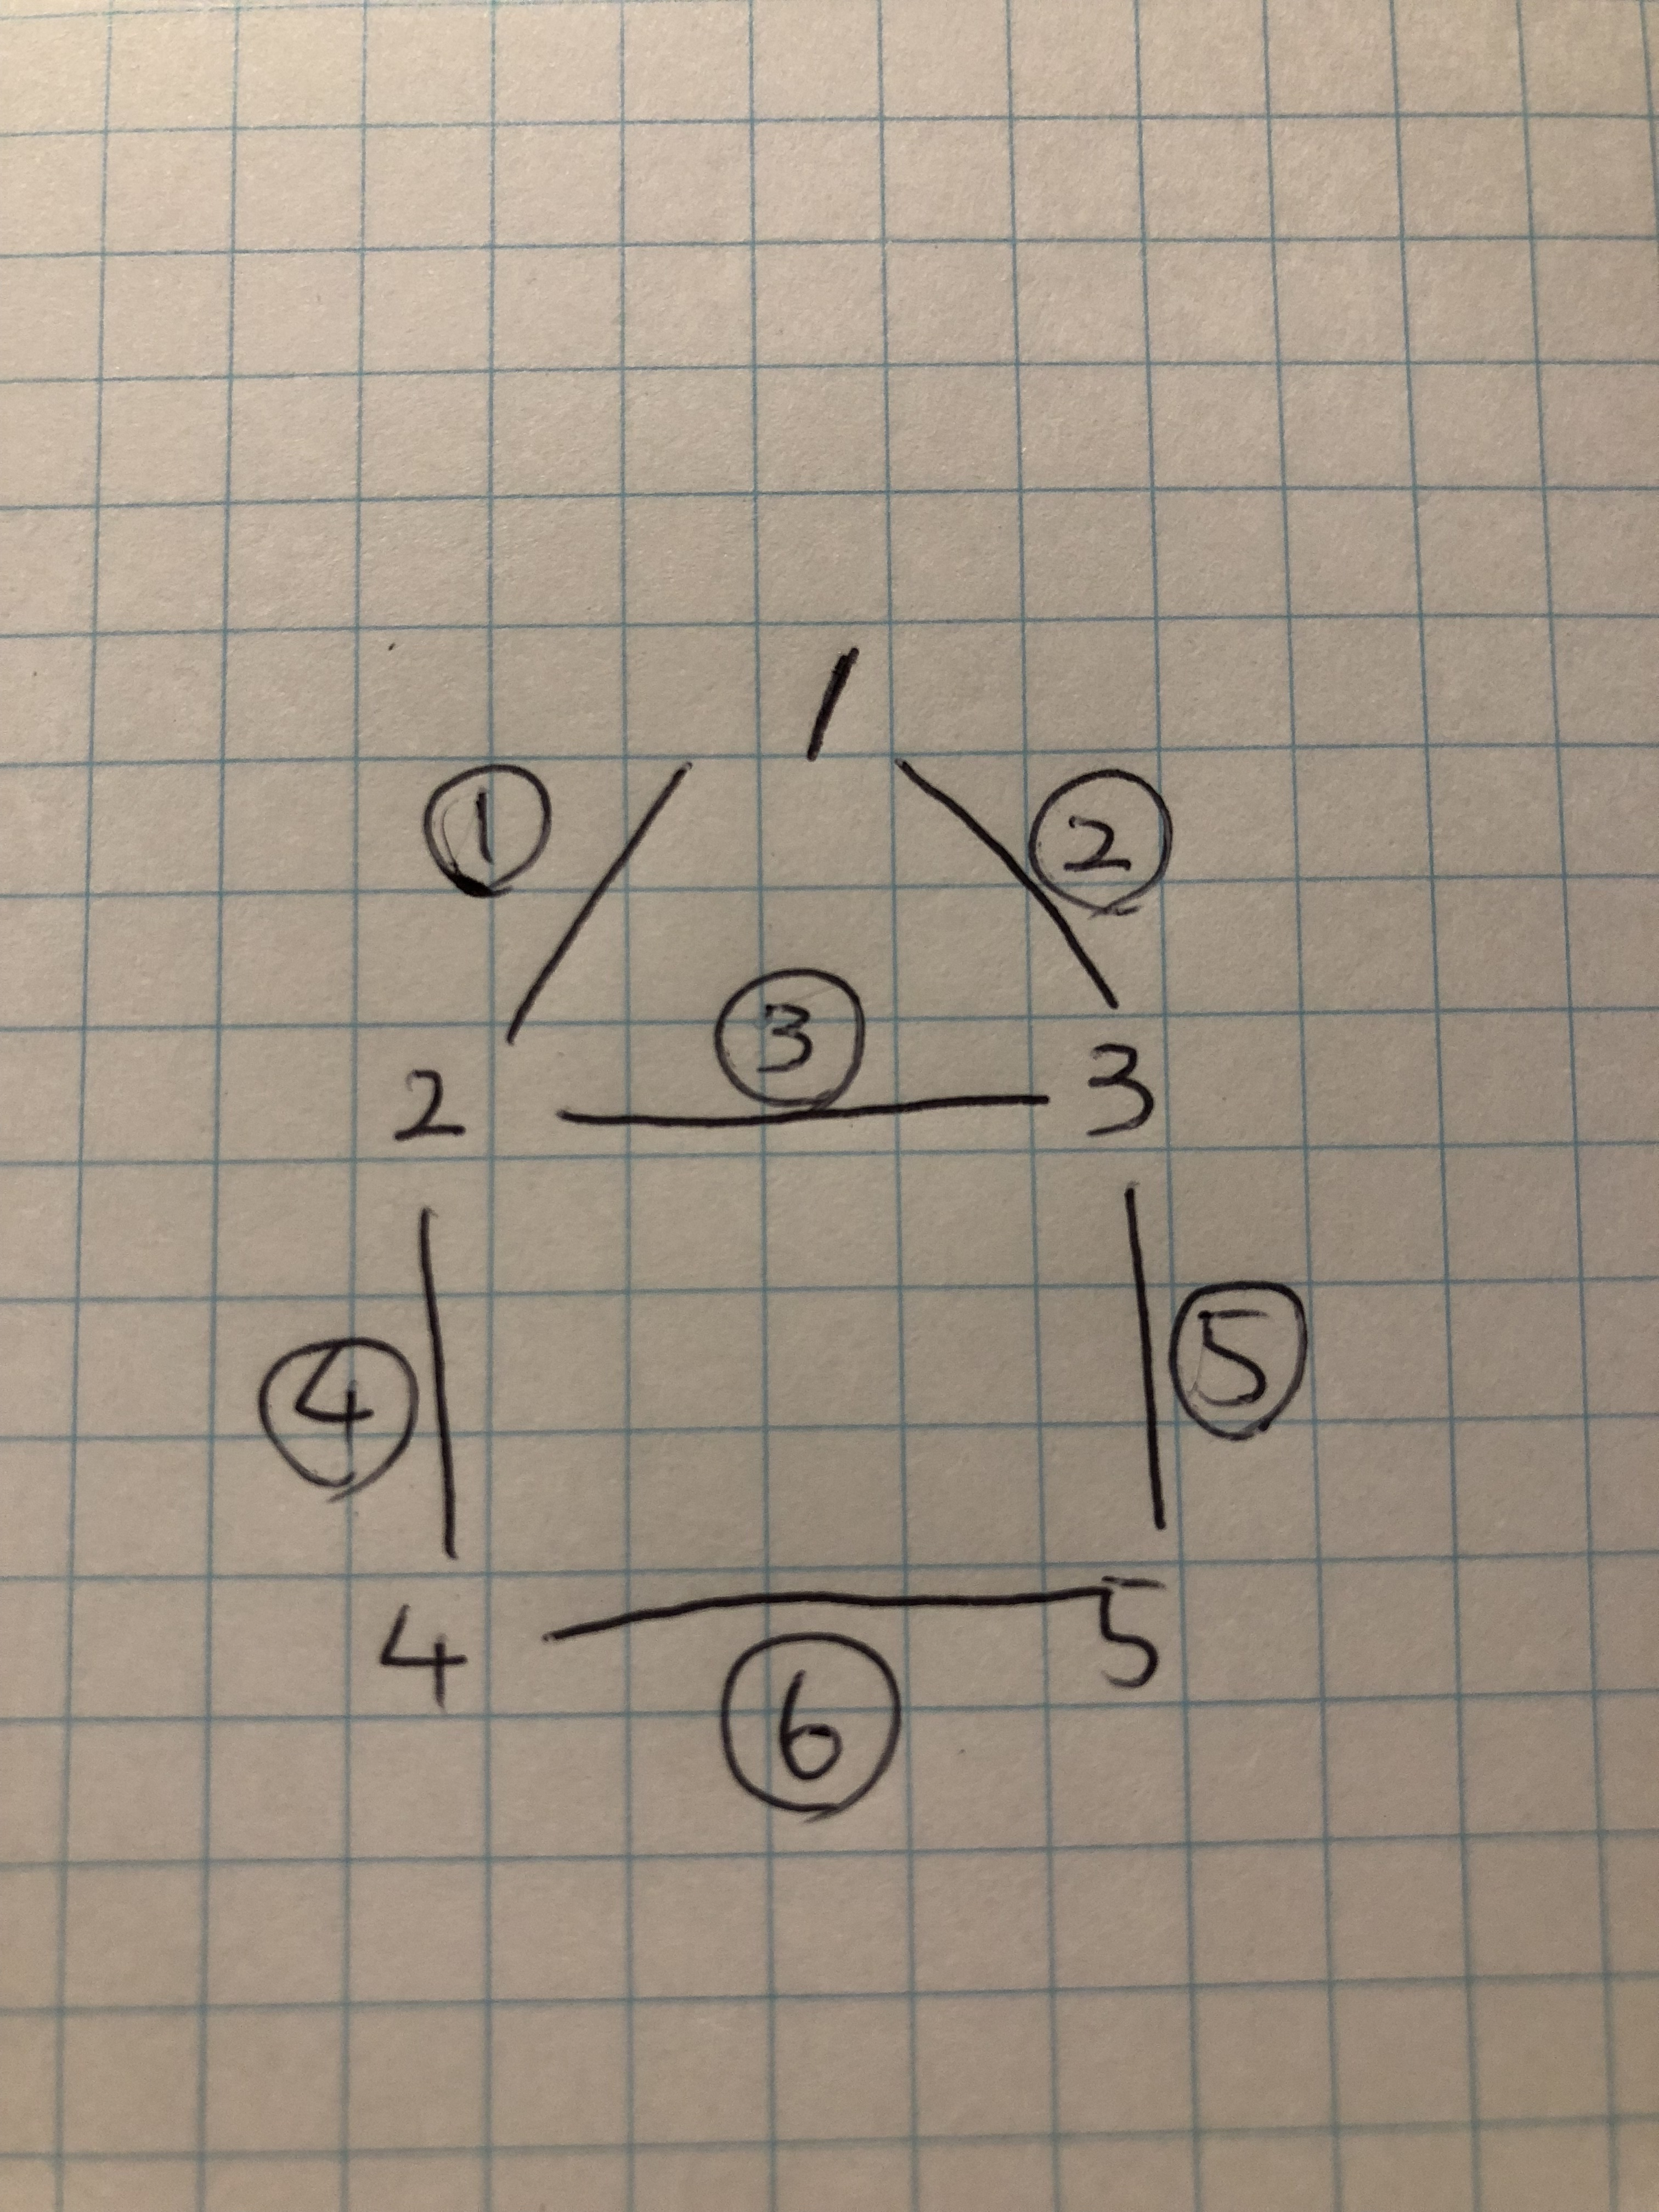
\includegraphics[width = 4cm]{画像/square.jpg}
    \caption{家型トラス構造:補強なし}
    \label{家1truss}
  \end{center}
\end{figure}

\begin{figure}[H]
  \begin{tabular}{cc}
    \begin{minipage}{0.5\hsize}
      \begin{center}
        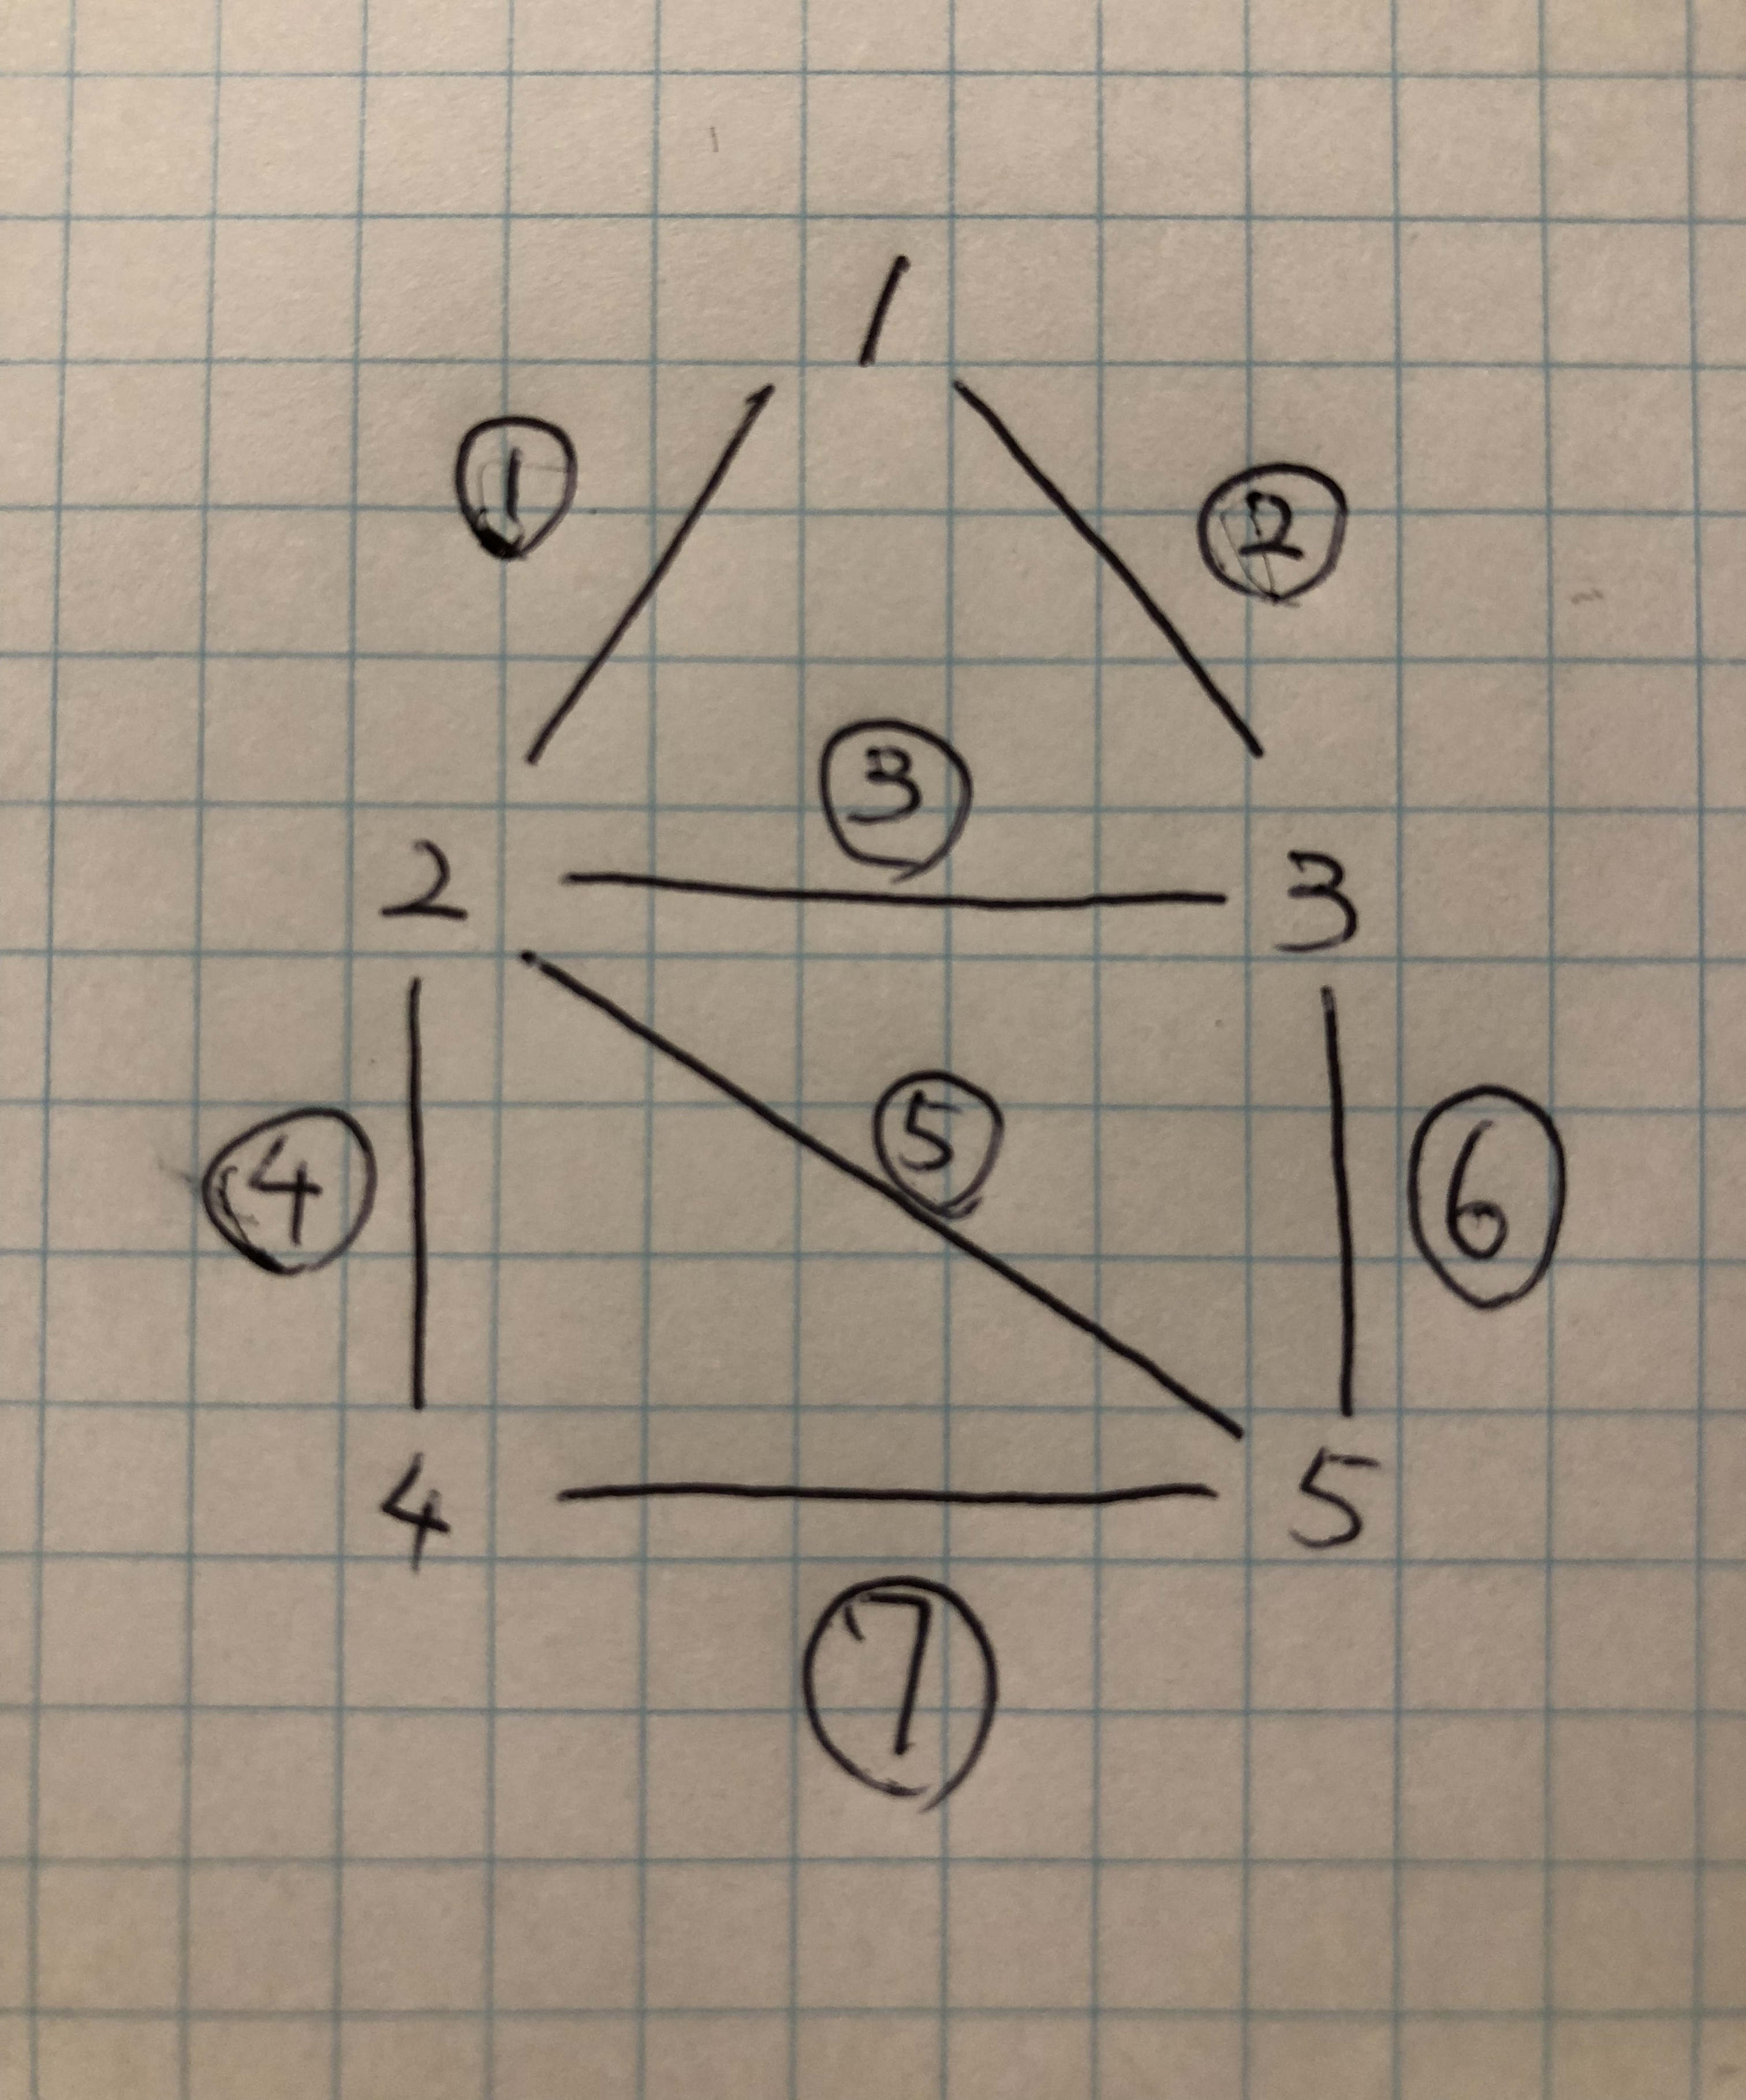
\includegraphics[width = 5cm]{画像/25.jpg}
        \caption{家型トラス構造:補強あり(A)}
        \label{家2truss}
      \end{center}
    \end{minipage}

    \begin{minipage}{0.5\hsize}
      \begin{center}
        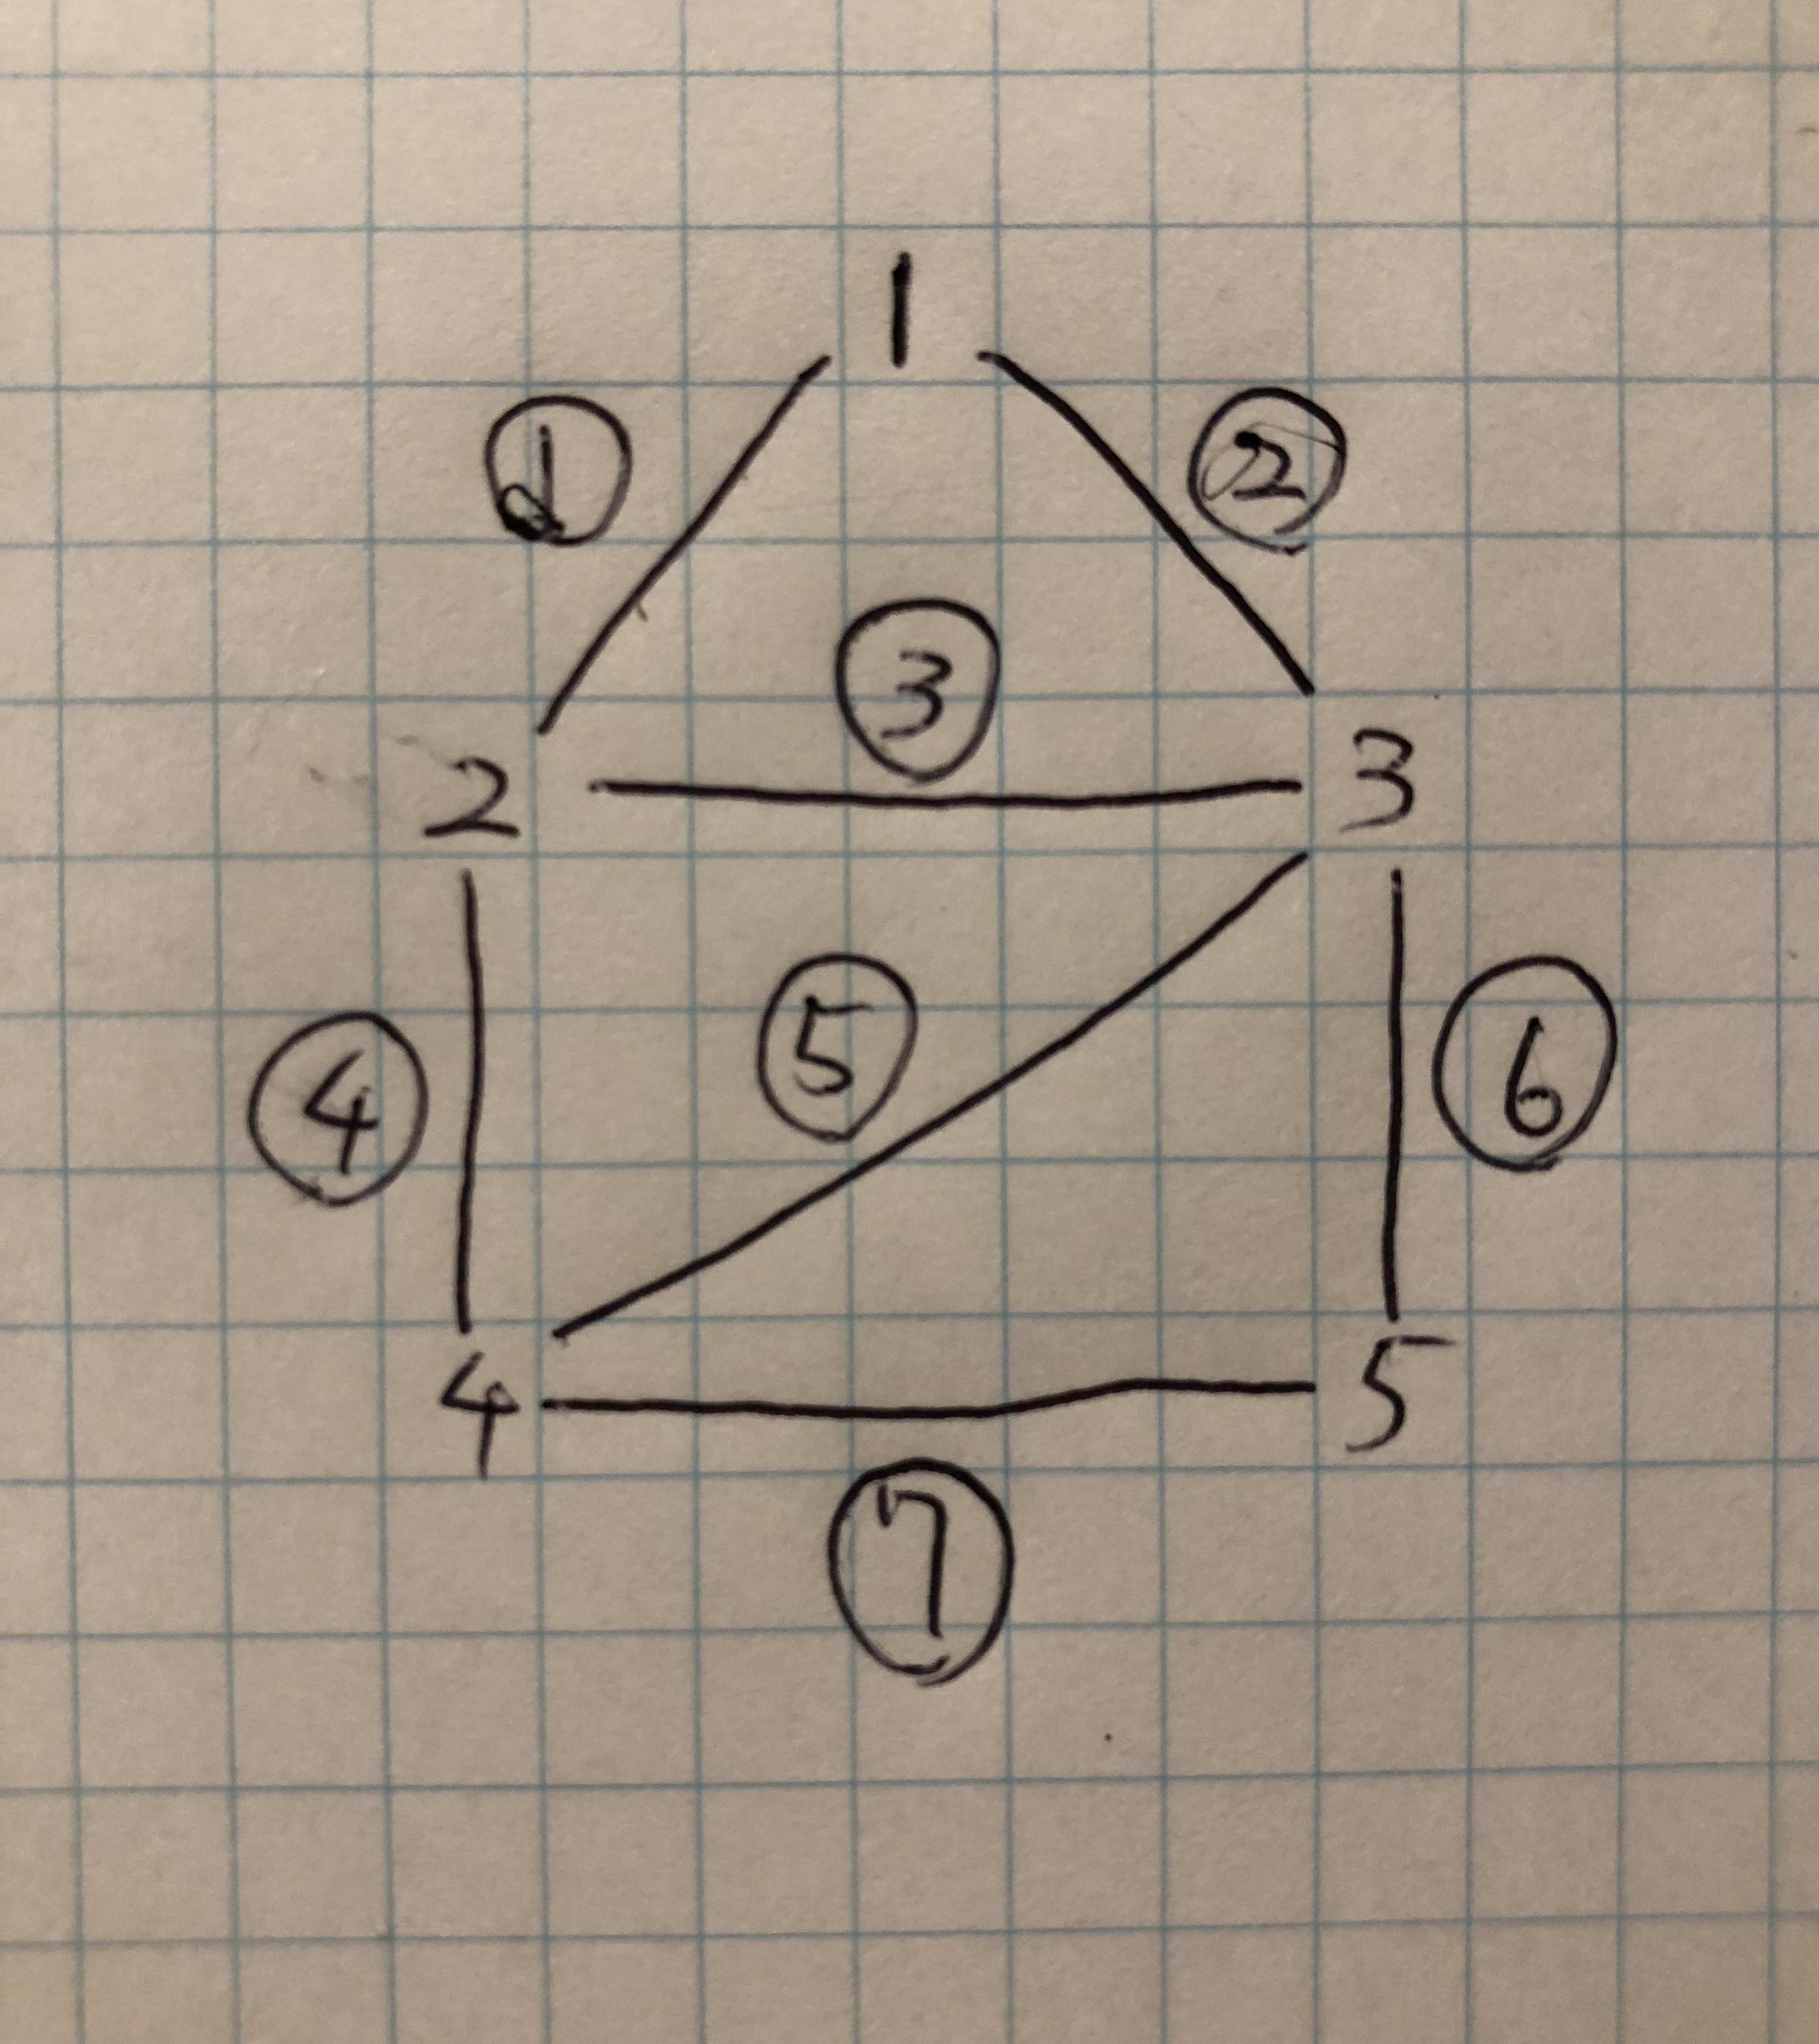
\includegraphics[width = 5cm]{画像/34.jpg}
        \caption{家型トラス構造:補強あり(B)}
        \label{家3truss}
      \end{center}
    \end{minipage}
  \end{tabular}
\end{figure}

\section{結果と考察}
3つのトラス構造を計算結果と可視化した図を以下に示す.
なお計算結果については付録に添付した.\\

\begin{figure}[H]
  \begin{center}
    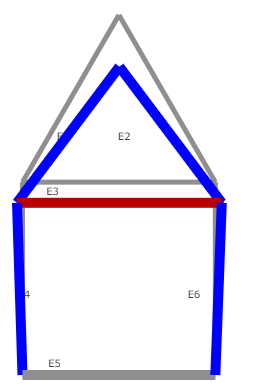
\includegraphics[width = 4cm]{画像/square.png}
    \caption{家型トラス構造:補強なしの可視化図}
    \label{家1}
  \end{center}
\end{figure}

\begin{figure}[H]
  \begin{tabular}{cc}
    \begin{minipage}{0.5\hsize}
      \begin{center}
        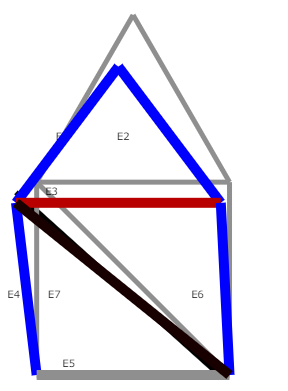
\includegraphics[width = 5cm]{画像/square25.png}
        \caption{家型トラス構造:補強あり(A)の可視化図}
        \label{家2}
      \end{center}
    \end{minipage}

    \begin{minipage}{0.5\hsize}
      \begin{center}
        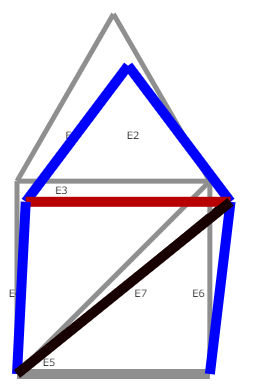
\includegraphics[width = 5cm]{画像/square34.png}
        \caption{家型トラス構造:補強あり(B)の可視化図}
        \label{家3}
      \end{center}
    \end{minipage}
  \end{tabular}
\end{figure}

\begin{figure}[H]
  \begin{center}
    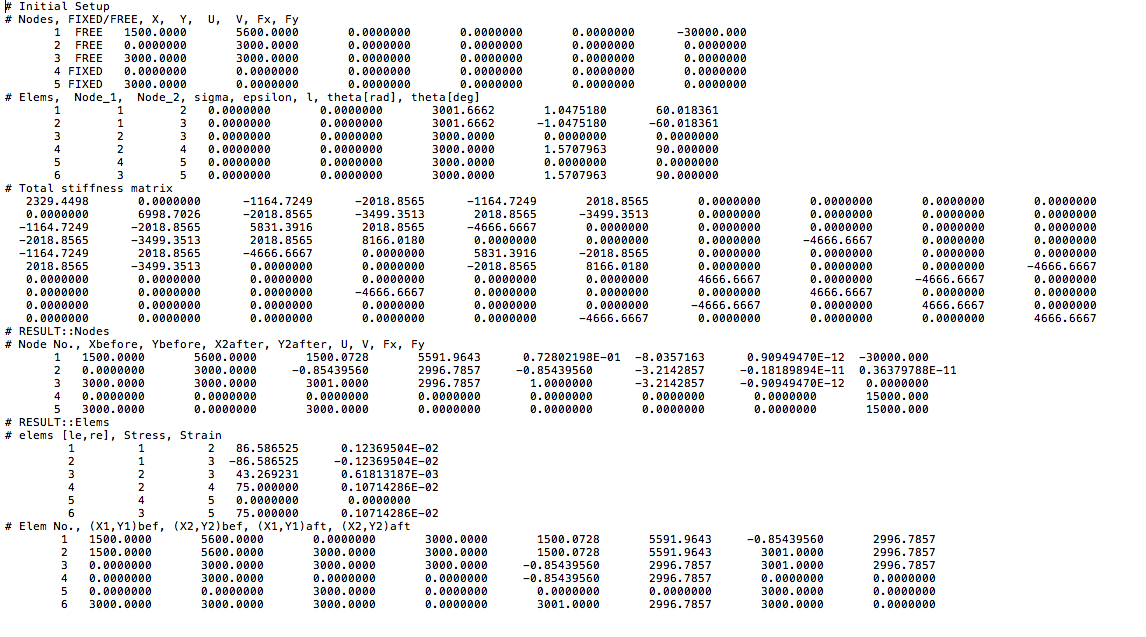
\includegraphics[width = 14cm]{画像/squareresult.png}
    \caption{家型トラス構造:補強なしの計算結果}
    \label{補強なし結果}
  \end{center}
\end{figure}

\begin{figure}[H]
  \begin{center}
    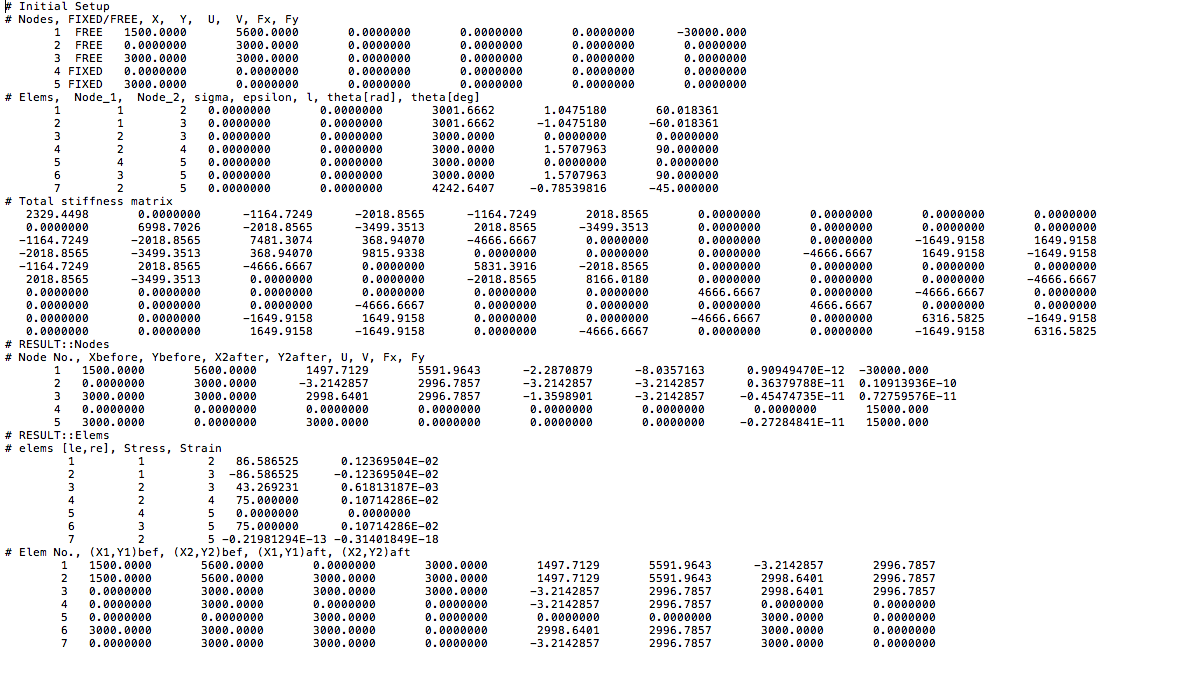
\includegraphics[width = 14cm]{画像/square25result.png}
    \caption{家型トラス構造:補強あり(A)の計算結果}
    \label{補強A結果}
  \end{center}
\end{figure}

\begin{figure}[H]
  \begin{center}
    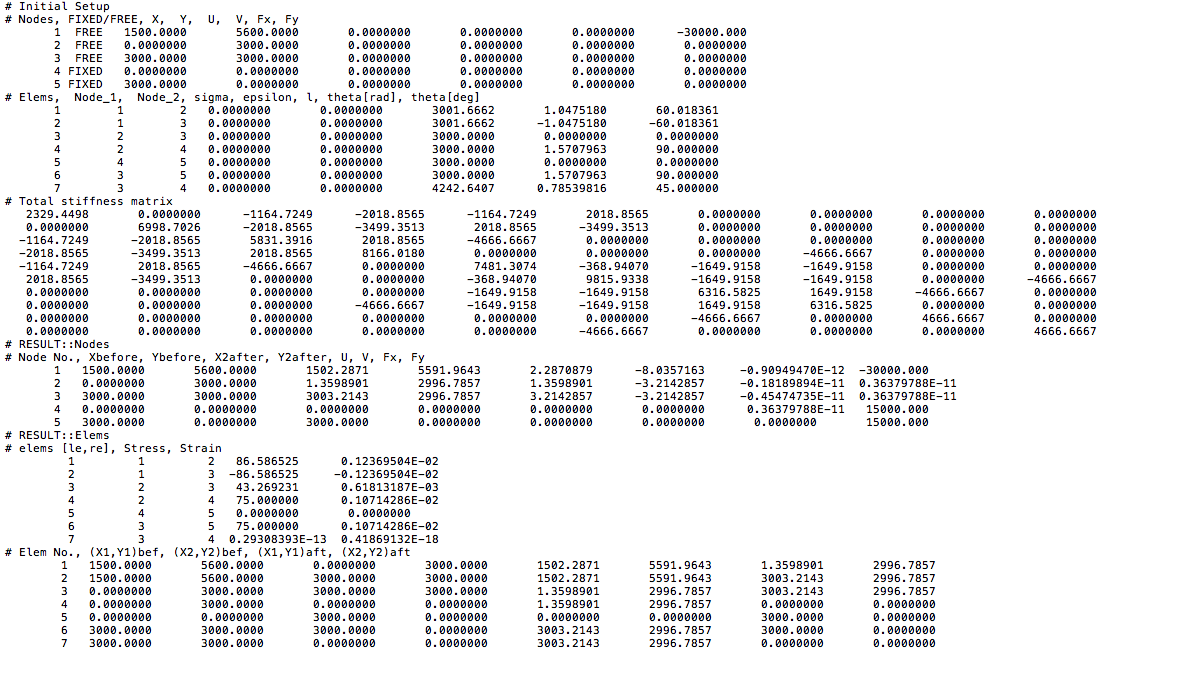
\includegraphics[width = 14cm]{画像/square34result.png}
    \caption{家型トラス構造:補強あり(B)の計算結果}
    \label{補強結果B}
  \end{center}
\end{figure}

\subsection{補強なし}
屋根,柱の部分は圧縮応力がかかっており,梁の部分には引張応力がかかっている.
歪みは小さく,応力も適度に分散しており,非常に安定した構造であることがわかる.
\subsection{補強あり(A)}
節点2,5に補強する要素を加えると,大きく左に傾いてしまっている.
屋根,柱の部分は圧縮応力がかかっており,梁の部分には引張応力,補強部分にはわずかな引張応力がかかっている.
補強なしと比べると応力が全体として大きくなり,バランスも悪くなっている.
\subsection{補強あり(B)}
節点3,4に補強する要素を加えると,大きく右に傾いてしまっている.
屋根,柱の部分は圧縮応力がかかっており,梁の部分には引張応力,補強部分にはわずかな引張応力がかかっている.
補強なしと比べると応力が全体として大きくなり,バランスも悪くなっている.
\subsection{まとめ}
補強を入れたことによって,逆に応力が大きくなる要素が生じ,不安定な構造になってしまった.
応力解析のレポート課題とこの実験を通して,安定した構造となるためには以下のような条件が挙げられる.
\begin{description}
  \item[荷重方向と反対方向の応力をもつ要素を多い]上から荷重がかかる場合には圧縮応力をもつ要素を多くもつ構造の方が歪みも応力も小さい.
  \item[左右対称である方が良い]左右の構造に偏りがあると,歪みや応力にも偏りが生まれてしまい,応力が大きくなったり,歪みが大きくなってしまう.
\end{description}
以上を通して,今回の課題では,補強あり(A)を右に,補強あり(B)を左にして組み合わせることで,左右対称で支え合う構造になり,安定した構造になるのではないかと考えられる.

\end{document}
